\documentclass{article}
\usepackage{graphicx}
\usepackage{amsmath}
\usepackage{float}
\usepackage[utf8]{inputenc}
\usepackage[ngerman]{babel}

\title{Projektdokumentation - Rechnernetzte \& Kommunikationssystem}
\author{Clemens Dehnert}
\date{Januar, 2024}

\begin{document}

\maketitle
\newpage

\tableofcontents
\newpage

\section{Aufgabenstellung}
Im Rahmen des Moduls "Rechnernetze und Kommunikationssysteme" war ein Beleg zu erstellen, welcher ein Java-Programm zur Datenübertragung zwischen zwei Computern beinhaltet. Dabei war zusätzlich eine Dokumentation anzufertigen, wobei theoretisches Wissen mit der Praxis abgeglichen wurde.

\section{Programm-Dokumentation}
Dieses Kapitel behandelt, welche Funktionen das Java-Programm bietet und welche Funktionen nicht umgesetzt wurden.

\subsection{Funktionalität}
Das Programm bietet folgende grundlegende Funkltionalitäten mit SW:
\begin{itemize}
  \item Funktion Ihres Clients + Server ohne Fehlersimulation OK 
  \item Funktion Ihres Clients + Server mit Fehlersimulation OK
  \item Funktion Ihres Clients + Server über Hochschulproxy (OK) Test über ./filetransfer Server 5555 100 0.2
  \item Funktion Ihres Clients + Hochschulserver ohne Fehlersimulation OK
  \item Funktion Ihres Clients + Hochschulserver mit Fehlersimulation OK
\end{itemize}

\vspace{1em}Es wurden folgende Aufgaben der Aufgabenstellung mit SW umgesetzt:
\begin{itemize}
  \item Aufruf des Clients OK 
  \item Aufruf des Servers OK
  \item Datei wird beim Empfänger korrekt benannt OK
  \item Ausgabe Datenrate OK
  \item Implementierung Protokoll OK
  \item Fehlerkorrektur OK
  \item Implementierung Protokoll OK
\end{itemize}

\vspace{1em}Folgende Klassen und Methoden stehen zur Verfügung:
\begin{itemize}
    \item FileCopy
    \begin{itemize}
        \item sendFile(): initiiert Senden der Datei
        \item handleConnection(): initiiert Warten auf Anfragen
    \end{itemize}
    \item FileTransfer
    \begin{itemize}
        \item file\_req(): teilt zu sendende Datei auf und gibt Teile der Datei in SW
        \item file\_init(): setzt aus SW kommende Dateiteile zusammen
    \end{itemize}
    \item SW
    \begin{itemize}
        \item data\_req(): sendet Daten aus FileTransfer
        \item data\_ind\_req(): wartet aus eingehende Daten
        \item closeConnection(): setzt Membervariablen der Servers zurück
    \end{itemize}
\end{itemize}

\begin{figure}[H]
    \centering
    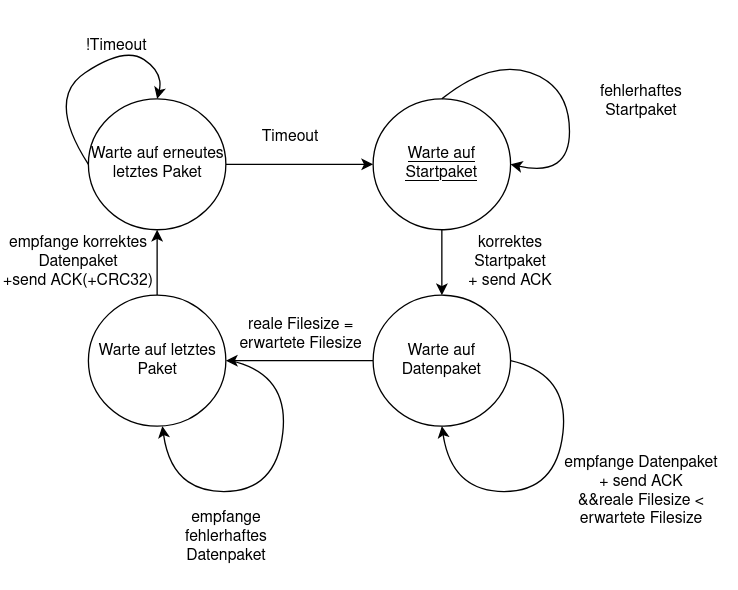
\includegraphics[width=0.8\linewidth]{Server_Zustandsdiagramm.png}
    \caption{Zustandsdiagramm Server}
    \label{fig:server}
\end{figure}

\begin{figure}[H]
    \centering
    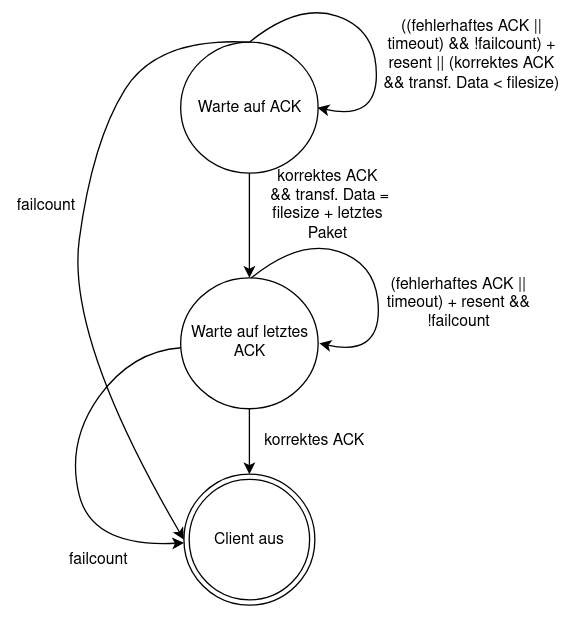
\includegraphics[width=0.6\linewidth]{Client_Zustandsdiagramm.png}
    \caption{Zustandsdiagramm Client}
    \label{fig:client}
\end{figure}

\subsection{Durchsatz in Theorie und Praxis}
Der maximale theoretisch erzielbare Durchsatz bei 10 Prozent Paketverlust und 10 ms Verzögerung beträgt:
\[\eta_{\text{max}} = \lim_{{T_p \to \infty}} \left( \frac{T_p}{{T_p + 2 \cdot T_a + T_{\text{ACK}}}} \cdot (1 - P_e)^2  \cdot R\right)\]
\[\eta_{\text{max}} = \lim_{{T_p \to \infty}} \left( \frac{T_p}{{T_p + 2 \cdot 0.01  + 0.01}} \cdot (1 - 0.1)^2 \cdot {\frac{1400}{1403}}\right)\]
\[\eta_{\text{max}} = 0.81\]

Der reale Durchsatz bei 10 Prozent Paketverlust und 10 ms Verzögerung beträgt:
\[\eta_{\text{real}} = \left( \frac{T_p}{{T_p + 2 \cdot T_a  + T_{\text{ACK}}}} \cdot (1 - P_e)^2 \cdot R\right)\]
\[\eta_{\text{real}} = \left( \frac{T_p}{{T_p + 2 \cdot 0.01  + 0.01}} \cdot (1 - 0.1)^2 \cdot {\frac{1400}{1403}} \right)\]
\[T_p = \left( \frac{(1400+3)\cdot 8}{315000} \right)\]
\[\eta_{\text{real}} = 0.44\]
Die Datenrate ergab sich aus Messungen.

Der gemessene Durchsatz ist geringer, als der theoretisch maximale Durchsatz. Das kann damit begründet werden, dass die Timeouts bei verlorengegangenen Paketen nicht optimal gesetzt sind.  

\subsection{Probleme}
Das Empfangen des CRC32 auf Seiten des Clients war kompliziert. Um der waitForAck()-Funktion in der Schicht SW zu signalisieren, dass sie das ACK-Paket des Servers mit dem CRC32 erhält, musste eine Membervariable verwendet war, wobei kein Boolean verfügbar war, wenn man nicht von der gegebenen Programmstruktur abweichen wollte.

\subsection{Limitierungen}
Es kann nur mit 'Stop and Wait' übertragen werden. Die Berechnung des Timeouts ist simpel, aber deshalb ist das Risiko, dass er ungünstig ist hoch. 

\subsection{Verbesserungsvorschläge}
Eine detailliertere Beschreibung zur Verwendung des Hochschulservers und Proxys wäre hilfreich. Des Weiteren wäre eine höhere Gewichtung des Belegs motivierender.
\newpage

\section{Lernportfolio}
Dieses Kapitel behandelt die persönlichen Lernfortschritte im Projekt. 

\subsection{Entwicklungsschritte}
Zu Beginn des Projektes war ein grundlegender Aufbau des Programms bereits gegeben. Das war eine sehr hilfreiche Grundlage. Es war dennoch eine recht lange Einarbeitungszeit nötig, um die Klassen und das Arbeiten in Schichten zu verstehen. Es hat sich als sinnvoll herausgestellt, in kleinen Schritten vorzugehen. Das Protokoll "Stop and Wait" wurde zuerst implementiert, wobei auf die Fehlerkorrektur zunächst verzichtet wurde. Als eine fehlerfreie Übertragung möglich war, wurde die Fehlerkorrektur implementiert, was sich als überraschend aufwendig herausstellte, da sich Bugs in dem mittlerweile etwas größerem Code nicht leicht finden ließen. Letztendlich wurden kleinere Features wie die Ausgabe der Datenrate oder die korrekte Dateibenennung für den Empfänger umgesetzt.   

\subsection{Lernfortschritte}
Die bereits vorhandenen Kommentare zur Funktionalität einzelner Funktionenköpfen hat die konkrete Implementierung wesentlich erleichtert. Deshalb haben sich nur selten Fragen zum Algorithmus aufgetan - anders die Frage, wie sich etwas in Java konkret implementieren lässt. Da Java nur sehr kurz im Modul Programmieren 2 behandelt wurde, war insbesondere die Bytemanipulation und das Arbeiten mit Arrays nicht trivial, aber mit den richtigen Klassen nach etwas Einarbeitung möglich.

Des Weiteren war das Arbeiten in Schichten etwas Ungewohntes, da man prinzipiell nur den Umgang mit Objekten in einer objektorientierten Programmiersprache gelehrt bekommt.  

Ein weiterer Lernaspekt war das Schreiben mit Latex. Hilfreich erwies sich dabei ChatGPT, was wesentlich schneller und präsize den passenden Befehl, den man sucht, liefert, als wenn man eine klassische Suchmaschine nutzt. 

\subsection{Misserfolge}
Das Protokoll "Go back N" wurde nicht umgesetzt. Grund dafür waren fehlende Zeit, aber auch Motivation, nachdem bereits eine mittlere zweistellige Anzahl an Stunden für Stop and wait aufgebracht wurde. Erschwerend kommt hinzu, dass der Beleg nur zu 30 Prozent in die Endnote eingeht. 
Nicht optimal lief noch, dass die Arbeit am Beleg die Zeit für die Vorbereitung der Seminare verringert hat. Sicherlich ist das eine Frage des Zeitmanagements, aber nach persönlichem Empfinden, erschwert die parallele Abarbeitung die Fokussierung wesentlich. 

\end{document}